%  LaTeX support: latex@mdpi.com
%  In case you need support, please attach all files that are necessary for compiling as well as the log file, and specify the details of your LaTeX setup (which operating system and LaTeX version / tools you are using).

% You need to save the "mdpi.cls" and "mdpi.bst" files into the same folder as this template file.

%=================================================================
\documentclass[agronomy,article,submit,moreauthors,pdftex,10pt,a4paper]{mdpi} 

%--------------------
% Class Options:
%--------------------
% journal
%----------
% Choose between the following MDPI journals:
% actuators, admsci, aerospace, agriculture, agronomy, algorithms, animals, antibiotics, antibodies, antioxidants, applsci, arts, atmosphere, atoms, axioms, batteries, behavsci, beverages, bioengineering, biology, biomedicines, biomimetics, biomolecules, biosensors, brainsci, buildings, carbon, cancers, catalysts, cells, challenges, chemosensors, children, chromatography, climate, coatings, computation, computers, condensedmatter, cosmetics, cryptography, crystals, data, dentistry, designs, diagnostics, diseases, diversity, econometrics, economies, education, electronics, energies, entropy, environments, epigenomes, fermentation, fibers, fishes, fluids, foods, forests, futureinternet, galaxies, games, gels, genealogy, genes, geosciences, geriatrics, healthcare, horticulturae, humanities, hydrology, informatics, information, infrastructures, inorganics, insects, instruments, ijerph, ijfs, ijms, ijgi, inventions, jcdd, jcm, jdb, jfb, jfmk, jimaging, jof, jintelligence, jlpea, jmse, jpm, jrfm, jsan, land, languages, laws, life, literature, lubricants, machines, magnetochemistry, marinedrugs, materials, mathematics, mca, mti, medsci, medicines, membranes, metabolites, metals, microarrays, micromachines, microorganisms, minerals, molbank, molecules, mps, nanomaterials, ncrna, neonatalscreening, nutrients, particles, pathogens, pharmaceuticals, pharmaceutics, pharmacy, philosophies, photonics, plants, polymers, processes, proteomes, publications, recycling, religions, remotesensing, resources, risks, robotics, safety, sensors, separations, sexes, sinusitis, socsci, societies, soils, sports, standards, sustainability, symmetry, systems, technologies, toxics, toxins, universe, urbansci, vaccines, vetsci, viruses, water
%---------
% article
%---------
% The default type of manuscript is article, but can be replaced by: 
% addendum, article, book, bookreview, briefreport, casereport, changes, comment, commentary, communication, conceptpaper, correction, conferencereport, expressionofconcern, meetingreport, creative, datadescriptor, discussion, editorial, essay, erratum, hypothesis, interestingimage, letter, newbookreceived, opinion, obituary, projectreport, reply, retraction, review, sciprints, shortnote, supfile, technicalnote
% supfile = supplementary materials
%----------
% submit
%----------
% The class option "submit" will be changed to "accept" by the Editorial Office when the paper is accepted. This will only make changes to the frontpage (e.g. the logo of the journal will get visible), the headings, and the copyright information. Also, line numbering will be removed. Journal info and pagination for accepted papers will also be assigned by the Editorial Office.
%------------------
% moreauthors
%------------------
% If there is only one author the class option oneauthor should be used. Otherwise use the class option moreauthors.
%---------
% pdftex
%---------
% The option pdftex is for use with pdfLaTeX. If eps figure are used, remove the option pdftex and use LaTeX and dvi2pdf.

%=================================================================
\firstpage{1} 
\makeatletter 
\setcounter{page}{\@firstpage} 
\makeatother 
\articlenumber{x}
\doinum{10.3390/------}
\pubvolume{xx}
\pubyear{2016}
\copyrightyear{2016}
\externaleditor{Academic Editor: name}
\history{Received: date; Accepted: date; Published: date}
%------------------------------------------------------------------
% The following line should be uncommented if the LaTeX file is uploaded to arXiv.org
%\pdfoutput=1

%=================================================================
% Add packages and commands here. The following packages are loaded in our class file: fontenc, calc, indentfirst, fancyhdr, graphicx, lastpage, ifthen, lineno, float, amsmath, setspace, enumitem, mathpazo, booktabs, titlesec, etoolbox, amsthm, hyphenat, natbib, hyperref, footmisc, geometry, caption, url, mdframed

%=================================================================
%% Please use the following mathematics environments:
 \theoremstyle{mdpi}
 \newcounter{thm}
 \setcounter{thm}{0}
 \newcounter{ex}
 \setcounter{ex}{0}
 \newcounter{re}
 \setcounter{re}{0}

 \newtheorem{Theorem}[thm]{Theorem}
 \newtheorem{Lemma}[thm]{Lemma}
 \newtheorem{Corollary}[thm]{Corollary}
 \newtheorem{Proposition}[thm]{Proposition}

 \theoremstyle{mdpidefinition}
 \newtheorem{Characterization}[thm]{Characterization}
 \newtheorem{Property}[thm]{Property}
 \newtheorem{Problem}[thm]{Problem}
 \newtheorem{Example}[ex]{Example}
 \newtheorem{ExamplesandDefinitions}[ex]{Examples and Definitions}
 \newtheorem{Remark}[re]{Remark}
 \newtheorem{Definition}[thm]{Definition}
%% For proofs, please use the proof environment (the amsthm package is loaded by the MDPI class).

%=================================================================
% Full title of the paper (Capitalized)
\Title{Growing Degree-days Accumulation and Trends in Phenological Stages of the Maize Billbug [\textit{Sphenophorus maidis} (Chittenden)] in Eastern Gamagrass [\textit{Tripsacum dactyloides} (L.) L.]}

% Authors, for the paper (add full first names)
\Author{Kundan Dhakal $^{1,}$* and Tim L. Springer $^{2}$}
% Authors, for metadata in PDF
\AuthorNames{Kundan Dhakal and Tim L. Springer}

% Affiliations / Addresses (Add [1] after \address if there is only one affiliation.)
\address{%
$^{1}$ \quad Oak Ridge Institute for Science and Education, Oak Ridge, TN 37830; \href{mailto:kundan.dhakal@ars.usda.gov}{kundan.dhakal@ars.usda.gov}\\
$^{2}$ \quad USDA, Agricultural Research Service, Southern Plains Range Research Station, 2000 18th Street, Woodward, Oklahoma 73801; \href{mailto:tim.springer@ars.usda.gov}{tim.springer@ars.usda.gov}}

% Contact information of the corresponding author
\corres{Correspondence: \href{mailto:kundan.dhakal@ars.usda.gov}{kundan.dhakal@ars.usda.gov}; Tel.: +1-(580) 256-7449}
%\href{mailto:kundan.dhakal@ars.usda.gov}{kundan.dhakal@ars.usda.gov}
% Current address and/or shared authorship
%\firstnote{Current address: Affiliation 3} 
%\secondnote{These authors contributed equally to this work.}

% Simple summary
%\simplesumm{}

% Abstract (Do not use inserted blank lines, i.e. \\) 
\abstract{The maize billbug, \textit{Sphenophoris maidis} (Chittenden) feeds on eastern gamagrass (\textit{Tripsacum dactyloides} (L.) L.), causing economic damage. We studied incidence of \textit{S. maidis} in a six-year-old eastern gamagrass establishment and influence of cumulative growing degree-days (cGDD) on the phenological stages of the pest for two years.Larval, pupal, and adult life stages of the billbug are described and illustrated. Based on growing degree-days, the \text{99\%} quantile for larvae, pupae, and adult maize billbugs was estimated between 1967.8–4234.6 cGDD.Very few pupae were recovered from field sampling, which we relate to short pupation period and weekly sampling interval in our study.  Findings of this study are helpful to formulate sustainable maize billbug management strategies.}

% Keywords
\keyword{maize billbug;  eastern gamagrass; life-cycle; growing degree-days.}

% The fields PACS, MSC, and JEL may be left empty or commented out if not applicable
%\PACS{J0101}
%\MSC{}
%\JEL{}

% If this is an expanded version of a conference paper, please cite it here: enter the full citation of your conference paper, and add $^\S$ in the end of the title of this article.
%\conference{}

%%%%%%%%%%%%%%%%%%%%%%%%%%%%%%%%%%%%%%%%%%
% Only for the journal Data:

%\dataset{DOI number or link to the deposited data set in cases where the data set is published or set to be published separately. If the data set is submitted and will be published as a supplement to this paper in the journal Data, this field will be filled by the editors of the journal. In this case, please make sure to submit the data set as a supplement when entering your manuscript into our manuscript editorial system.}

%\datasetlicense{license under which the data set is made available (CC0, CC-BY, CC-BY-SA, CC-BY-NC, etc.)}

%%%%%%%%%%%%%%%%%%%%%%%%%%%%%%%%%%%%%%%%%%
\begin{document}

%%%%%%%%%%%%%%%%%%%%%%%%%%%%%%%%%%%%%%%%%%
%% Sections that are not mandatory are listed as such. The section titles given are for Articles. Review papers and other article types have a more flexible structure. 

%% Only for the journal Gels: Please place the Experimental Section after the Conclusions

%%%%%%%%%%%%%%%%%%%%%%%%%%%%%%%%%%%%%%%%%%

\section{Introduction}

Eastern gamagrass (\textit{Tripsacum dactyloides} (L.) L. [Poaceae]), a distant relative of maize (\textit{Zea mays} L.), is a warm-season perennial C${_4}$ bunchgrass distributed throughout the eastern, central, and southern United States \cite{ref-barkworth07,hitchcock}. The grass is primarily used for forage and hay and was recognized by Magoffin as early as 1843 for its productivity and high-quality palatable forage \cite{hitchcock1899}. There is considerable variation in eastern gamagrass leaf widths, plant heights and widths, disease resistance, forage quality, maturity date, yield, and plant architecture---which is helpful for developing geographically and edaphically widely adapted cultivars \cite{salon2000}. Some of the present eastern gamagrass cultivars include: Pete, Iuka IV, Jackson, Medina Highlander, and Verl \cite{springer04,springer06}. Because of difficulty with establishment, low seed production potential, and overgrazing---declines in its natural population have been reported \cite{rechenthin1951}. Eastern gamagrass is a valued forage for haying and grazing, it provides multiple ecosystem services, such as, phytoremediation \cite{euliss08}, soil amelioration, and soil conservation \cite{gilker02}; and for these reasons, eastern gamagrass has attracted considerable attention among stakeholders in forage and livestock industry \cite{springer04}. Since the eastern gamagrass production area been increasing over the years, pest and diseases are also becoming more abundant and problematic \cite{springer04}.


The billbugs (\textit{Sphenophorus} spp.) are found throughout the continental United States and have been reported to be harmful for range grasses, cool and warm-season turf grasses, and agricultural crops \cite{sattertjwait1931}. Vaurie’s “Revision of the Genus \textit{Sphenophorus} in the United States and Mexico” in 1951 is the most comprehensive taxonomic reference for this genus. Most billbugs are univoltine species, which overwinter as pupae. The genus contains 71 species, with 64 being indigenous to North America \cite{vaurie}. Eleven billbug species infest managed turfgrass in North America, and at least four species are associated with turfgrass in the Midwest, which include bluegrass billbug (\textit{S. parvulus} Gyllenhal), hunting billbug (\textit{S. venatus vestitus}), southern corn billbug (\textit{S. callosus}), lesser billbug (\textit{S. minimus}), and Timothy billbug (\textit{S. inaequalis}) \cite{kuhn12,richmond}. Attention was first given to billbug species during late 1960s when an outbreak of the \textit{S. parvulus} damaged residential lawns across several states \cite{tashiro70}. Often multiple billbug species co-occur infesting turfgrass and identification of larvae to the species level based solely on association with the presence of adults can be difficult and unreliable \cite{duffy18}.

Some of the pests found to affect eastern gamagrass include \textit{Diatraea mitteri} Solis \cite{solis15} and maize billbug [\textit{Sphenophorus maidis} (Chittenden)] \cite{springer06,maas03}. The maize billbug species was first described by Dr. F. H. Chittenden; and as early as 1854 it was  reported to be very destructive to corn (\textit{Zea mays} L.) \cite{kelly1911}. Eastern gamagrass was reported as a host plants of maize billbug by Satterthwait \cite{sattertjwait1931}. Springer et al. \cite{springer04_1} estimated a potential eastern gamagrass yield loss of 1.32 Mg ha$^{-1}$ due to maize billbug infestation, which could significantly reduce forage production and stand longevity. This is equivalent to a loss in eastern gamagrass hay production between 7.4–56.8 USD ha$^{-1}$, with an average of 27.1 USD ha$^{-1}$ (estimates based on 40 USD Mg$^{-1}$)\cite{springer04_1}.



Because so much remains unknown about eastern gamagrass’s pests’ population and life cycle dynamics, predicting outbreak is extremely challenging. Thick and creeping root stocks of the eastern gamagrass provide shelter to various pests. Although eastern gamagrass is considered relatively free of insects, pests, and plant pathogens \cite{krizek04}, taxonomic proximity of eastern gamagrass to maize makes it more susceptible to disease and pests in maize \cite{springer06,maas03}. Adult maize billbugs feed on young shoots of eastern gamagrass, leaving a transverse feeding pattern. Female maize billbugs feed at the base of the culm for ovipositioning and once the eggs hatch, the larvae feed voraciously producing a cavity at the base of the culm, thereby causing extensive damage to the culm base which results in the death of the culm \cite{springer03}. Because knowledge of the life cycle of the maize billbug in eastern gamagrass will be useful for developing cultural practices for control, research was conducted to understand the life stages of development of the maize bill bug in eastern gamagrass. We present and overview of maize billbug ecology, with a focus on extent of seasonal phenology of maize billbug population in eastern gamagrass and to formulate strategies to minimize its damage to eastern gamagrass.

\section{Materials and Methods}

\subsection{Site description and weather conditions}


This study was conducted at the USDA-ARS Southern Plains Range Research Station (SPRRS), Woodward, OK (36\degree 25’N 99\degree 24’W, elevation 615 m asl), during the year 2003 and 2004. Eastern gamagrass germplasm ‘FGT-1’ \cite{Dewald96} were transplanted in the field in 1996, and spaced at 1.1 m. The soil of the experimental plot was a Devol fine sandy loam (Thermic Typic Haplustalfs). Each year, the plants were burned in mid-March and atrazine (2-chloro-4-ethylamino-6-isopropylamino-1,3,5-triazine) at the rate of 1.68 ai ha$^{-1}$ was applied between 7–14 days of burning for weed control. Nitrogen fertilizer in the form of urea was applied to soil at 70 kg N ha$^{-1}$. No insecticides were applied in the field. Beginning in January 2003, four plant crowns were randomly selected and dug each week throughout the year for maize billbug sampling. Plant shoots of the sampled materials were segregated into reproductive and vegetative shoots and the shoots were dissected to determine the presence of maize billbug larvae, pupae, and adult maize billbugs (Figure \ref{fig:MB}). Detailed methods of sampling are published in Springer, et al. \cite{springer11}.The rainfall and daily high and low temperatures and 30–year average climate normal were obtained from an automated weather station located approximately 1 km from the study site (Table \ref{table1}). 

\begin{figure}
  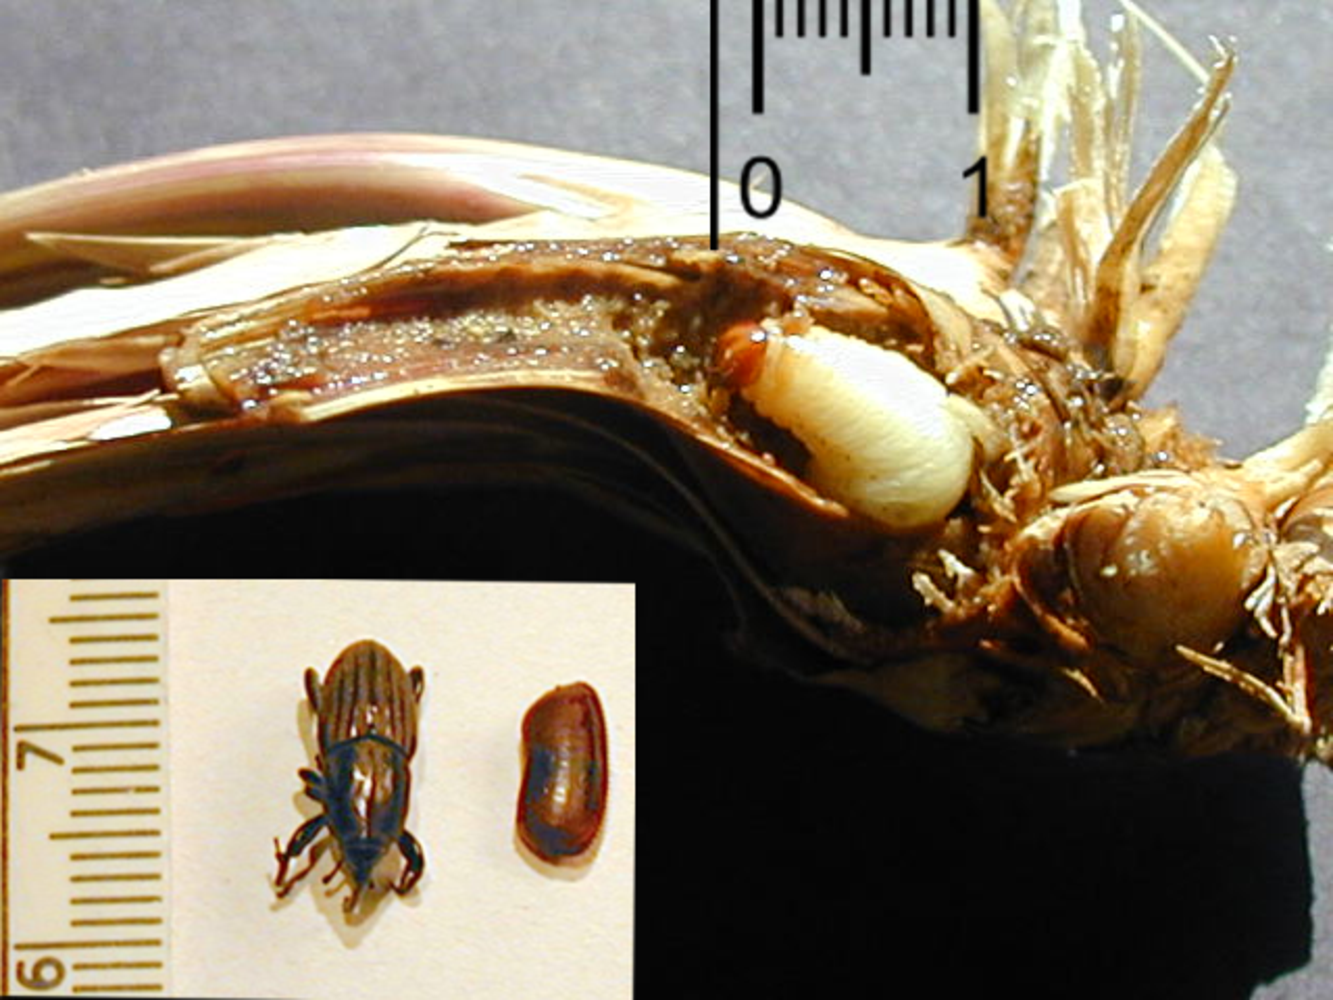
\includegraphics[width=450 pt]{bilbug.pdf}
  \caption{Larvae of \textit{Sphenophorus maidis} (top) within a feeding cavity located at the base of eastern gamagrass [\textit{Tripsacum dactyloides} (L.) L.] culm; adult and pupae in the inset (scale bar in \textit{cm}).}
  \label{fig:MB}
\end{figure}

%\begin{tabularx}{\textwidth}{X|l}

\begin{table}

\captionsetup[table]{labelsep=space, 
         justification=raggedright, singlelinecheck=off}

\caption{Monthly mean maximum and minimum temperatures, and monthly total rainfall in 2003 and 2014 in comparison with the 30-year mean (1981-2010) for Woodward, Oklahoma, USA.}
\label{table1}
\begin{tabular}{llllllllllll} 
\toprule
\multirow{2}{*}{\textbf{Month}} & \multicolumn{3}{c}{\textbf{2003}}                                                                                                                                                                                                      & ~ & \multicolumn{3}{c}{\textbf{2004}}                                                                                                                                                                                                      & ~ & \multicolumn{3}{c}{\textbf{30-year mean}}                                                                                                                                                                                             \\ 
\cmidrule{2-2}\cmidrule{3-3}\cmidrule{4-4}\cmidrule{6-6}\cmidrule{7-7}\cmidrule{8-8}\cmidrule{10-10}\cmidrule{11-11}\cmidrule{12-12}
                       & \multicolumn{1}{c}{\begin{tabular}[c]{@{}c@{}}\textbf{Max T}\\~(\textbf{\degree C})\end{tabular}} & \multicolumn{1}{c}{\begin{tabular}[c]{@{}c@{}}\textbf{Min T}\\~(\textbf{\degree C})\end{tabular}} & \multicolumn{1}{c}{\begin{tabular}[c]{@{}c@{}}\textbf{Rain}\\ \textbf{(mm)}\end{tabular}} & ~ & \multicolumn{1}{c}{\begin{tabular}[c]{@{}c@{}}\textbf{Max T}\\ (\textbf{\degree C})\end{tabular}} & \multicolumn{1}{c}{\begin{tabular}[c]{@{}c@{}}\textbf{Min T}\\~(\textbf{\degree C})\end{tabular}} & \multicolumn{1}{c}{\begin{tabular}[c]{@{}c@{}}\textbf{Rain}\\~\textbf{(mm)}\end{tabular}} & ~ & \multicolumn{1}{c}{\begin{tabular}[c]{@{}c@{}}\textbf{Max T}\\(\textbf{\degree C})\end{tabular}} & \multicolumn{1}{c}{\begin{tabular}[c]{@{}c@{}}\textbf{Min T} \\(\textbf{\degree C})\end{tabular}} & \multicolumn{1}{c}{\begin{tabular}[c]{@{}c@{}}\textbf{Rain}\\\textbf{(mm)}\end{tabular}}  \\ 
\bottomrule
Jan                    & 10                                                                       & -4                                                                       & 2                                                                       & ~ & 10                                                                       & -4                                                                       & 32                                                                      & ~ & 9                                                                       & -6                                                                       & 13                                                                      \\
Feb                    & 8                                                                        & -4                                                                       & 10                                                                      & ~ & 10                                                                       & -3                                                                       & 34                                                                      & ~ & 12                                                                      & -3                                                                       & 25                                                                      \\
Mar                    & 17                                                                       & 2                                                                        & 47                                                                      & ~ & 19                                                                       & 6                                                                        & 78                                                                      & ~ & 17                                                                      & 2                                                                        & 46                                                                      \\
Apr                    & 23                                                                       & 8                                                                        & 35                                                                      & ~ & 21                                                                       & 8                                                                        & 50                                                                      & ~ & 23                                                                      & 7                                                                        & 53                                                                      \\
May                    & 26                                                                       & 12                                                                       & 37                                                                      & ~ & 30                                                                       & 15                                                                       & 1                                                                       & ~ & 27                                                                      & 13                                                                       & 102                                                                     \\
Jun                    & 28                                                                       & 17                                                                       & 111                                                                     & ~ & 30                                                                       & 18                                                                       & 168                                                                     & ~ & 32                                                                      & 18                                                                       & 81                                                                      \\
Jul                    & 36                                                                       & 22                                                                       & 1                                                                       & ~ & 32                                                                       & 20                                                                       & 47                                                                      & ~ & 35                                                                      & 21                                                                       & 66                                                                      \\
Aug                    & 35                                                                       & 21                                                                       & 92                                                                      & ~ & 31                                                                       & 18                                                                       & 95                                                                      & ~ & 34                                                                      & 19                                                                       & 74                                                                      \\
Sep                    & 26                                                                       & 14                                                                       & 75                                                                      & ~ & 30                                                                       & 16                                                                       & 29                                                                      & ~ & 29                                                                      & 15                                                                       & 58                                                                      \\
Oct                    & 23                                                                       & 9                                                                        & 10                                                                      & ~ & 22                                                                       & 9                                                                        & 86                                                                      & ~ & 24                                                                      & 8                                                                        & 48                                                                      \\
Nov                    & 15                                                                       & 3                                                                        & 16                                                                      & ~ & 13                                                                       & 3                                                                        & 120                                                                     & ~ & 16                                                                      & 1                                                                        & 36                                                                      \\
Dec                    & 11                                                                       & -2                                                                       & 17                                                                      & ~ & 13                                                                       & -2                                                                       & 3                                                                       & ~ & 10                                                                      & -4                                                                       & 20                                                                      \\
\bottomrule
\end{tabular}
\end{table}
%\end{tabularx}


\subsection{Cumulative Growing Degree-Days}

Several empirical and experimental evidences have shown that seasonal biology and population dynamics of insects are primarily regulated by temperature. Growing Degree-Days (GDD) is a commonly used measure of thermal accumulation, as the mechanistic link between ambient air temperature, which serves as a proxy for growing conditions within a region, and species phenology. GDD explicitly constraints the thermal limits within which growth is possible. Therefore, GDD has been extensively used to predict phenology by agriculturists, entomologists, and ecologists \cite{higley86}. We used the following canonical equation (\ref{eq:1}) to calculate growing degree-days (GDD) for each year using the weather data measured at the SPRRS station.

\begin{equation}
\label{eq:1}
GDD= \sum \left [ \frac{T_{max}+T_{min}}{2} -T_{base}\right ]
\end{equation}

Where T$_{max}$ is the daily maximum air temperature, T$_{min}$ is the daily minimum air temperature, and T$_{base}$ is the temperature below which the process of the species does not progress. We used a minimum threshold of 10\degree C and a maximum of 30\degree C to calculate GDD from a biofix date of January 1 using the daily maximum and minimum ambient temperature recorded for the site. All analyses were conducted using SAS software, version 9.4 (SAS Institute Inc., Cary, NC, USA). We used PROC UNIVARIATE to obtain descriptive statistics for cumulative growing degree-days (cGDD) for each life stage 




\section{Results and Discussion}

Larvae, pupae, and adult comprised 30.2, 8.3 and \text{61.4\%} of the total sampled population respectively. The \text{99\%} quantile for larvae, pupae, and adult maize billbugs was estimated between 1967.8–3514.3 cGDD for 2003 and 2040.9–4234.6 for 2004 (Table \ref{table2}). The first captures of \textit{S. maidis’}s larvae, pupae, and adult were recorded as early as DOY 169, 190, and 7 for 2003 and DOY 175, 189, and 14 for 2004 respectively. Larval stage in maize billbug ranges from 32–75 days depending upon the weather and host plants \cite{hayes1916}. Similarly, a three-year study in maize billbug under laboratory conditions reported varying larval stages (33–70), with an average larval period of 49.15 days \cite{cwright1929}. In our study, larvae were found between DOY 169–239 (Jun 17–Aug 26) which translates to 900–1957 cGDD. This is similar to that reported by Hayes \cite{hayes1916} for corn in southern Kansas (June through early September) and Carrwright \cite{cwright1929} in South Carolina. Histogram of the cGDD shows that peak larva occurrence was observed around 1200 cGDD in 2003 and 1500 cGDD in 2004 (Figures \ref{fig:f1} and \ref{fig:f2}). 



\begin{figure}
  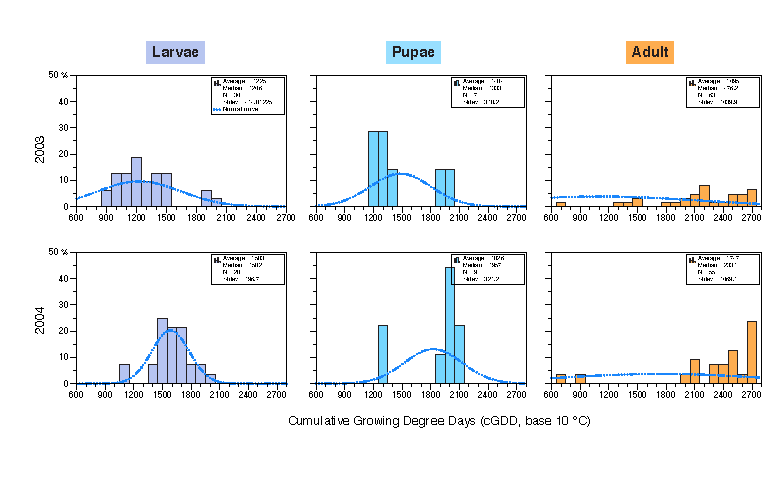
\includegraphics[width=\linewidth]{Fig1.eps}
  \caption{Histogram of cumulative growing degree-days (base 10 \degree C) based on occurrence of maize billbig (\textit{S. maidis}’s) larvae, pupae, and adult population for 2003 and 2004 at Woodward, Oklahoma.}
  \label{fig:f1}
\end{figure}



Pupae were collected between 1150–1450 cGDD and 1850–2150 cGDD both years, between 7 June and 9 Sept. The length of the pupation stage in corn can vary annually, ranging between 9–30 days, depending upon the weather \cite{hayes1916}. Pupation period is short in a dry season and long in a wet season \cite{hayes1916}. Likewise, Cartwright \cite{cwright1929} reported a three-year average pupal period of 9.86 days (minimum 8 days, maximum 15 days) under laboratory conditions. Hayes \cite{hayes1916} reported maize billbug’s pupae in maize between mid-July through early September. Similarly, Cartwright \cite{cwright1929} reported finding maize billbug from mid-July through mid-October. In general, pupae were difficult to recover. As stated earlier, pupation in corn varies between 9 and 30 days depending upon the weather, it may be possible that the pupation period is less for eastern gamagrass due to the fact that our sampling interval was every seven days and very few pupae were recovered during sampling. Adult maize billbugs were collected throughout the year during both seasons (Figures \ref{fig:f1} and \ref{fig:f2}).

\begin{figure}
  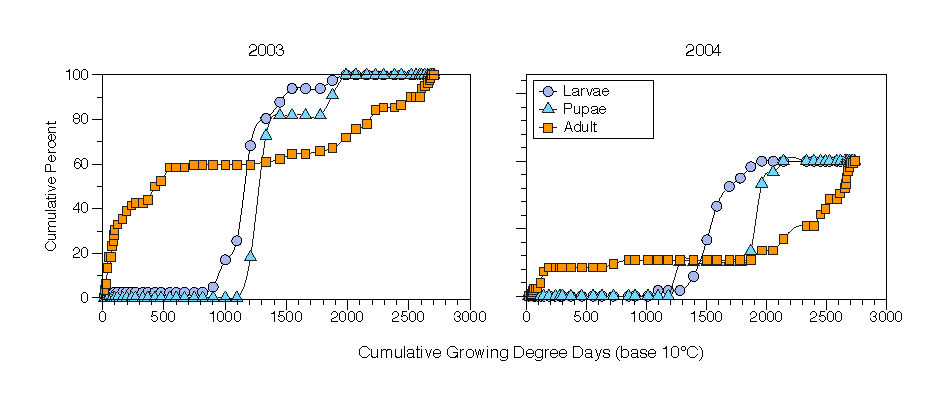
\includegraphics[width=\linewidth]{Fig2.eps}
  \caption{Cumulative population patterns of different development periods of \textit{S. maidis} (base 10 \degree C, after January 1).}
  \label{fig:f2}
\end{figure}

Larvae, pupae, and adult populations were greater in reproductive shoots compared with vegetative shoots. No pupae were collected in vegetative shoots. However, larvae and adult populations in the reproductive shoot were 1.28 and 3.2 times greater than their corresponding population in vegetative shoots (Figure \ref{fig:f3}). 




The nutritive value of eastern gamagrass is superior to corn, with lipid and protein contents being 1.5 and 3 times greater than that of corn respectively \cite{bargman89}. The amount of total nonstructural carbohydrate (TNC) in eastern gamagrass are highest during the winter dormant season and least during May and June \cite{dewald_kd}. A study conducted from 1993 through 1997 at the USDA-ARS SPRRS quantified the nutritive value of eastern gamagrass and found varying levels of nitrogen content; ranging from 2.3–3.1\text{\%}(14.6–19.6\text{\%} crude protein) in May to 0.8–1.2\text{\%}(5.3–7.6\text{\%} crude protein) in August \cite{gillen99}. It is known that high-protein diet allows for rapid development of larvae compared with than larvae surviving on low-protein diet, for e.g., Woods \cite{woods99} reported that fifth-instar Manduca sexta caterpillars reared on a high–protein diet (17.7\text{\%} casein by dry weight) grew 20\text{\%} more rapidly than caterpillars reared on a low-protein diet (5.9\text{\%} casein by dry weight). Similarly, Karowe and Martin \cite{karowe89} demonstrated that growth and survivorship of southern armyworm (Spodoptera erodania), prior to the onset of the fifth instar, were dependent upon the amount of protein diet. They reported that diets with 3.4–4.7\text{\%} nitrogen (20.9–30.5\text{\%} crude protein) resulted in the highest larval dry weight and survivorship (96–100\text{\%}) weight. Therefore, \textit{S. maidis} larvae appear to time their onset of stage and stabilize their relative growth rate when protein availability is relatively higher in eastern gamagrass.


\begin{figure}
  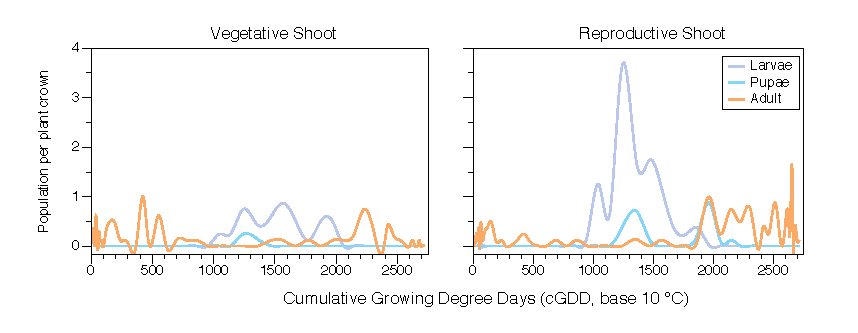
\includegraphics[width=\linewidth]{Fig3.eps}
  \caption{Frequency of maize billbug population (\textit{Sphenophorus maidis}) in eastern gamagrass reproductive and vegetative shoots, measured in Woodward, OK in 2003 and 2004. }
  \label{fig:f3}
\end{figure}


Adults are strong and vigorous, having few natural enemies. Adults remain protected during most part of their existence, either inside the plant crown or under the dead plant materials in the field. They can also survive underwater for several days in case of heavy rains and field flooding. On average eggs incubate somewhere between 8–12 days. Dry weather expedites eggs development thereby shortening the incubation period, whereas wet weather prolongs the development time \cite{hayes20}. 

Development of resistant eastern gamagrass cultivars with fine stems and leaves and tougher plant tissues, paired with IPM control strategies could be effective. Dupuy and Ramirez \cite{dupuy16} did a review on the biology and control of billbugs and described several cultural, biological, and chemical control methods for billbug management, with most focus on turfgrass. Due to lack of systemic insecticides labeled for eastern gamagrass and the  sheltered feeding habit of maize billbug, it  will be extremely difficult to control \cite{kuhn12}. Application of insecticides would be cost prohibitive and the cheapest and most effective means of maize billbug control is crop rotation \cite{cwright1929}. Natural enemies of maize billbug include \textit{Anaphoidea calandrae} Gahan that feed on their eggs, \textit{Cerceris bicornuta}, a wasp, that prey on adult maize billbug and take them to its nest for feeding its larvae, and parasitic fungus that cause mortality at any stage of its growth \cite{vaurie}.



% \usepackage{booktabs}


\begin{table}
 \begin{threeparttable}
\caption{Putative life-stages of the maize billbug [\textit{Sphenophorus maidis} (Chittenden)]}
\label{table2}
\begin{tabular}{lllllll} 
\toprule
~                        &                                &                                  & \multicolumn{1}{c}{cGDD\tnote{$\ddagger$}}     &                              & \multicolumn{2}{c}{cGDD\tnote{$\dagger$}}                                    \\ 
\cmidrule{4-4}\cmidrule{6-6}\cmidrule{7-7}
\multicolumn{1}{c}{Year} & \multicolumn{1}{c}{Life Stage} & \multicolumn{1}{c}{ \textit{n} } & \multicolumn{1}{c}{Mean $\pm$ SD} & \multicolumn{1}{c}{Quantile} & \multicolumn{1}{c}{Observed} & \multicolumn{1}{c}{Estimate}  \\ 
\bottomrule
2003                     & Larvae                         & 30                               & 1304 $\pm$ 285.3                   & 99                           & 1986.9                       & 1967.8                        \\
                         & Pupae                          & 7                                & 1483 $\pm$ 318.2                   & 99                           & 1986.9                       & 2224.1                        \\
                         & Adult                          & 63                               & 1095 $\pm$ 1039.9                  & 99                           & 2688.1                       & 3514.3                        \\
                         &                                &                                  &                              &                              &                              &                               \\
2004                     & Larvae                         & 28                               & 1583 $\pm$ 196.7                   & 99                           & 1957.2                       & 2040.9                        \\
                         & Pupae                          & 9                                & 1826 $\pm$ 321.2                   & 99                           & 2137.5                       & 2573.2                        \\
                         & Adult                          & 55                               & 1747 $\pm$ 1069.1                  & 99                           & 2732.5                       & 4234.6                        \\
\bottomrule
\end{tabular}
\begin{tablenotes}
			\small
            
            
\vspace{5 pt} 
            
            \item{$\ddagger$} Cumulative growing degree-days (cGDD) were calculated from 1 January and were calculated as cumulative number of degrees the average daily temperature meets the predetermined threshold, a base temperature of 10 \degree C and a maximum temperature of 30 \degree C.
            \vspace{7 pt} 
            \item{$\dagger$} Observed, the observed percentage of the observations in each quantile interval; Estimated, the estimated percentage of the population that falls into each quantile interval (estimated from the fitted normal distribution).
           
        \end{tablenotes}
\end{threeparttable}
\end{table}
\section{Conclusions}

The following summary is based largely upon observations made on the SPRRS station in Woodward, Oklahoma, but we believe that the same observations would be valid in the Southern Great Plains region. The developmental findings of our study suggest that lower threshold temperatures in maize billbug are likely to restrict its larval and pupal population under current climatic parameters. Adult population occur throughout the season. We believe, for optimal management strategy of billbug population, a spatio-temporal analysis will be necessary to establish a sound understanding and prediction of billbug seasonal activity. In addition, novel methods for studying the development from egg to adult under laboratory settings are imperative to fully understand the life-cycle of the pest and unravel information on sex ratio, female lifespan and fecundity, as well as larval biology.

Some of the control strategies include preventive application of contact and systemic insecticides targeting overwintering adult population before they oviposition during the spring. Burning of the eastern gamagrass residue in the spring followed by nitrogen fertilizer application could also be helpful in controlling maize billbug. Our study will be useful in improving the maize billbug’s scouting efficiency and forecasting of the seasonal occurrence of maize billbug in eastern gamagrass. In conclusion, we still have a fragmentary understanding of the maize billbug, creating demand for more research in all areas of its biology. Since the experiment was conducted in a field condition, it was harder to keep records of larval instars and their moulting because of the limited population encountered technical expertise in properly discriminating larval stages. Further research is needed in order to enlighten the underinvestigated life-cycle stages and its activity at various phenological stages and for the development of control and management mechanism that fits well with an IPM approach.


\vspace{6pt} 


%%%%%%%%%%%%%%%%%%%%%%%%%%%%%%%%%%%%%%%%%%
\acknowledgments{This research was supported in part by an appointment to the Agricultural Research Service (ARS) Research Participation Program administered by the Oak Ridge Institute for Science and Education (ORISE) through an interagency agreement between the U.S. Department of Energy (DOE) and the U.S. Department of Agriculture (USDA). ORISE is managed by ORAU under DOE contract number DE-SC0014664. All opinions expressed in this paper are the author's and do not necessarily reflect the policies and views of USDA, ARS, DOE, or ORAU/ORISE.  All programs and services of the USDA are offered on a nondiscriminatory basis, without regard to race, color, national origin, religion, sex, age, marital status, or handicap.  Thanks are extended to Darby Baker, William Cooper, Emalee Friend, David Maas, and Dana Smith for their assistance during the course of this research.}

%%%%%%%%%%%%%%%%%%%%%%%%%%%%%%%%%%%%%%%%%%
\authorcontributions{T. L. Springer conceived and designed the experiment; K. Dhakal and T. L. Springer analyzed the data and wrote the paper.}

%%%%%%%%%%%%%%%%%%%%%%%%%%%%%%%%%%%%%%%%%%
\conflictofinterests{The authors declare no conflict of interest.} 



%%%%%%%%%%%%%%%%%%%%%%%%%%%%%%%%%%%%%%%%%%
\bibliographystyle{mdpi}

%=====================================
% References, variant A: internal bibliography
%=====================================
\renewcommand\bibname{References}
\begin{thebibliography}{999}

% Reference 1
\bibitem{ref-barkworth07}
Barkworth, M.E.; Anderton, L.K.; Capels, K.M.; Long, S.; Piep, M.B. \textit{Manual of grasses for North America}. University Press of Colorado: \textbf{2007}.

% Reference 2
\bibitem{hitchcock}
Hitchcock, A.S. \textit{Manual of the grasses of the United States}. 2nd \textit{ed}. Revised by A. Chase. USDA: U.S. Gov. Print Office, Washington DC, \textbf{1950}; Vol. Misc. Publ. 200.

% Reference 3
\bibitem{hitchcock1899}
Hitchcock, A.S.; Clothier, G.L. \textit{Native agricultural grasses of Kansas}. Experiment Station, Kansas State Agricultural College: Manhattan, Kan., \textbf{1899}.

% Reference 4
\bibitem{salon2000}
Salon, P.R.; Dewald, C.L. In \textit{Eastern gamagrass breeding in New York and Oklahoma}, The Second Eastern Native Grass Symposium, Beltsville, Maryland, November 17–19, 2000; Ritchie, J.C.; Dickerson, J.A.; Ritchie, C.A., Eds. USDA-Agriculture Research Service, and USDA-Natural Resources Conservation Service: Beltsville, Maryland, 2000.

% Reference 5
\bibitem{springer04}
Springer, T.L.; Dewald, C.L. Eastern gamagrass and other tripsacum species. In \textit{Warm-season (C$_4$) grasses}, Moser, L.E.; Burson, B.L.; Sollenberger, L.E., Eds. American Society of Agronomy, Crop Science Society of America, Soil Science Society of America: Madison, WI, \textbf{2004}; pp. 955–973.


% Reference 6
\bibitem{springer06}
Springer, T.L.; Dewald, C.L.; Sims, P.L.; Gillen, R.L.; Louthan, V.H.; Cooper, W.J.; Taliaferro, C.M.; Maura, C.; Pfaff, S.; Wynia, R.L., et al. Registration of ‘Verl’ eastern gamagrass. \textit{Crop Science} \textbf{2006}, \textit{46}, 477–478.

% Reference 7
\bibitem{rechenthin1951}
Rechenthin, C.A. Range grasses in the southwest: Eastern gamagrass, texas cupgrass, Pan American balsomscale and smooth cordgrass. \textit{Cattleman} \textbf{1951}, \textit{38}, 110-112.

% Reference 8
\bibitem{euliss08}
Euliss, K.; Ho, C.H.; Schwab, A.P.; Rock, S.; Banks, M.K. Greenhouse and field assessment of phytoremediation for petroleum contaminants in a riparian zone. \textit{Bioresource Technology} \textbf{2008}, \textit{99}, 1961–1971.

% Reference 9
\bibitem{gilker02}
Gilker, R.E.; Weil, R.R.; Krizek, D.T.; Momen, B. Eastern gamagrass root penetration in adverse subsoil conditions. \textit{Soil Sci Soc Am J} \textbf{2002}, \textit{66}, 931–938.
% Reference 10
\bibitem{sattertjwait1931}
Satterthwait, A.F. Key to known pupae of the genus \textit{Calendra}, with host-plant and distribution notes. \textit{Annals of the Entomological Society of America }\textbf{1931}, \textit{24}, 143–172.

% Reference 11
\bibitem{vaurie}
Vaurie, P. Revision of the genus \textit{Calandra} (formerly \textit{Sphenophorus}) in the United States and Mexico (\textit{Coleoptera}, \textit{Curculionidae}) \textbf{1951}; pp 31–186.

% Reference 12
\bibitem{kuhn12}
Kuhn, W.R.; Youngman, R.R.; Wu, S.; Laub, C.A. Ecology, taxonomy, and pest management of billbugs (Coleoptera: \textit{Curculionidae}) in orchardgrass of Virginia. \textit{Journal of Integrated Pest Management }\textbf{2013}, \textit{4}, 1–5.

% Reference 13
\bibitem{richmond}
Richmond, D. Managing billbugs in turfgrass. Purdue Extension.

% Reference 14
\bibitem{tashiro70}
Tashiro, H.; Personius, K.E. Current status of the bluegrass billbug and its control in western New York home lawns. \textit{Journal of Economic Entomology} \textbf{1970}, \textit{63}, 23–29.

% Reference 15
\bibitem{duffy18}
Duffy, A.G.; Powell, G.S.; Zaspel, J.M.; Richmond, D.S. Billbug (Coleoptera: Dryophthoridae: \textit{Sphenophorus} spp.) seasonal biology and DNA-based life stage association in Indiana turfgrass. \textit{J Econ Entomol }\textbf{2018}, \textit{111}, 304–313.

% Reference 16
\bibitem{solis15}
Solis, M.A.; Metz, M.A.; Scheffer, S.J.; Lewis, M.L.; Kula, R.R.; Springer, T.L. A new cryptic species of \textit{Diatraea} (Lepidoptera: Crambidae: \textit{Crambinae}) feeding on eastern gamagrass and a novel host association with a braconid (hymenoptera) in the United States. \textit{Annals of the Entomological Society of America} \textbf{2015}, \textit{108}, 648–659.

% Reference 17
\bibitem{maas03}
Mass, D.; Springer, T.L.; Arnold, D. Occurrence of the maize billbug, sphenophorus maidis in eastern gamagrass. \textit{Southwestern Entomologist }\textbf{2003}, \textit{28}, 150–152.

% Reference 18
\bibitem{kelly1911}
Kelly, O.G. The maize billbug. In Papers on cereal and forage insects, Howard, L.O., Ed. U.S. Department of Agriculture, Bureau of Entomology: Washington, Government Printing Office, \textbf{1911}; Vol. Bulletin No. 95.

% Reference 19
\bibitem{springer04_1}
Springer, T.L.; Sims, P.L.; Gillen, R.L. In Estimates of forage yield loss in eastern gamagrass due to shoot boring insects, The 2004 Conference of the American Forage Grassland Council (AFGC), Roanoke, VA, June 12–16, \textbf{2004}; Cassida, K., Ed. Roanoke, VA, pp 333–336.

% Reference 20
\bibitem{krizek04}
Krizek, D.T.; Solis, M.A.; Touhey, P.A.; Ritchie, J.C.; Millner, P.D. Rediscovery of the southern cornstalk borer: A potentially serious pest of eastern gamagrass and strategies for mitigation. In \textit{Proceedings of the 3rd Eastern Native Grass Symposium}, The North Carolina Botanical Garden, Chapel Hill, North Carolina, 2004; Randall, J.; Burns, J.C., Eds. Omnipress, Madison, WI: The North Carolina Botanical Garden, Chapel Hill, North Carolina, pp 56–62.

% Reference 21 
\bibitem{springer03}
Springer, T.L.; Mass, D.L.; Gillen, R.L.; Sims, P.L. The maize billbug and \textit{Diatreaea }spp. In \textit{Insects affecting the seed production of eastern gamagrass}. Fifth International Herbage Seed Conference, Gatton, Australia, 2003; Loch, D.S., Ed. The University of Queensland, Gatton Campus: Gatton, Australia.

% Reference 22
\bibitem{Dewald96}
Dewald, C.L.; Kindiger, B. Registration of FGT-1 eastern gamagrass germplasm. \textit{Crop Science} \textbf{1996}, \textit{36}, 219–220.

% Reference 23
\bibitem{springer11}
Springer, T.L.; Puterka, G.J.; Maas, D.L.; Thacker, E.T. The southern cornstalk borer (\textit{Diatraea crambidoides }(Grote), Lepidoptera: \textit{Crambidae}) A new pest of eastern gamagrass (\textit{Tripsacum dactyloides} (L.) l., Poaceae). \textit{Journal of the Kansas Entomological Society} \textbf{2011}, \textit{84}, 209–216.

% Reference  24
\bibitem{higley86}
Higley, L.G.; Pedigo, L.P.; Ostlie, K.R. Degday - A program for calculating degree-days, and assumptions behind the degree-day approach. \textit{Environmental Entomology} \textbf{1986}, \textit{15}, 999–1016.

% Reference 25
\bibitem{hayes1916}
Hayes, W.P. A study of the life-history of the maize bill-bug. \textit{Journal of Economic Entomology} \textbf{1916}, \textit{9}, 120–130.

% Reference 26
\bibitem{cwright1929}
Carrwright, O.L. The maize billbug in South Carolina (\textit{Calendra maidis} Chittn.); Clemson Agricultural College: Clemson College, South Carolina, \textbf{1929}.

% Reference 27
\bibitem{bargman89}
Bargman, T.J.; Hanners, G.D.; Becker, R.; Saunders, R.M.; Rupnow, J.H. Compositional and nutritional evaluation of eastern gamagrass (\textit{Tripsacum dactyloides} (l.) l.), a perennial relative of maize (\textit{Zea mays }L.). \textit{LWT - Food Science and Technology }\textbf{1989}, \textit{22}, 208–212.

% Reference 28
\bibitem{dewald_kd}
Dewald, C.L.; Sims, P.L. Seasonal vegetative establishment and shoot reserves of eastern gamagrass. \textit{Journal of Range Management} \textbf{1981}, \textit{34}, 300–304.

% Reference  29
\bibitem{gillen99}
Gillen, R.L.; Berg, W.A.; Dewald, C.L.; Sims, P.L. Sequence grazing systems on the Southern Plains. \textit{Journal of Range Management }\textbf{1999}, \textit{52}, 583–589.

% Reference 30
\bibitem{woods99}
Woods, H.A. Patterns and mechanisms of growth of fifth-instar \textit{Manduca sexta} caterpillars following exposure to low- or high-protein food during early instars. \textit{Physiol Biochem Zool} \textbf{1999}, \textit{72}, 445–454.

% Reference 31
\bibitem{karowe89}
Karowe, D.N.; Martin, M.M. The effects of quantity and quality of diet nitrogen on the growth, efficiency of food utilization, nitrogen budget, and metabolic rate of fifth-instar \textit{Spodoptera eridania} larvae (Lepidoptera: \textit{Noctuidae}). \textit{Journal of Insect Physiology }\textbf{1989}, \textit{35}, 699–708.

% Reference 32
\bibitem{hayes20}
Hayes, W.P. The maize billbug or elephant bug (\textit{Sphenophorus maidis}, Chittn.); Topeka, Kansas, \textbf{1920}.

% Reference 33
\bibitem{dupuy16}
Dupuy, M.M.; Ramirez, R.A. Biology and management of billbugs (Coleoptera: \textit{Curculionidae}) in turfgrass. \textit{J Integr Pest Manag} \textbf{2016}, \textit{7}, 6.

\end{thebibliography}

\end{document}

